\section{Related Works}

\subsection{Audio Language Model}

The success of Large Language Models (LLMs) has sparked a significant trend in leveraging language foundation models for audio generation tasks \cite{rubenstein2023audiopalm,zhang2024speechlm,wu2023decoder,wu2023speechgen,yang2023uniaudio,chen2023lauragpt}. Audio, much like language, consists of variable-length sequences, making it well-suited for modeling with language foundation models. One pioneering method, AudioLM \cite{borsos2023audiolm}, employs a multi-stage strategy to harness the predictive capabilities of foundation models for generating tokens unconditionally. This approach involves predicting semantic tokens from various conditions (e.g., phonemes, text descriptions, MIDI) in the initial stage, followed by transforming them into acoustic tokens through coarse-to-fine modeling, ultimately generating the waveform. Representative systems such as SPEAR-TTS \cite{kharitonov2023speak} for speech synthesis and MusicLM \cite{agostinelli2023musiclm} for music generation have also been proposed. However, the two-stage process can lead to complexity in training and suboptimal performance due to the separate development of semantic and acoustic tokens, leading to error accumulation.

Conversely, recent advancements have shown that methods employing a single-stage language model outperform two-stage approaches. For example, VALL-E \cite{wang2023neural} utilizes an autoregressive (AR) model to predict the first token and a non-autoregressive (NAR) model to estimate the residual tokens, demonstrating superior performance compared to AudioLM. Similarly, MusicGen \cite{copet2024simple} employs a single-stage transformer language model and incorporates a delay pattern strategy for efficient token interleaving, achieving better results than MusicLM. Other notable works include CLAM-TTS \cite{kim2024clam}, VoiceCraft \cite{peng2024voicecraft}, and UniAudio \cite{yang2023uniaudio}.

Despite recent advancements, directly modeling the intricate low-level acoustic fluctuations with an LLM poses challenges. LLMs are primarily designed for processing natural language, which is inherently rich in semantics. In order to overcome this limitation, we propose X-Codec, a novel enhancement that aims to enrich semantic processing within acoustic codecs. By doing so, we aim to improve the overall performance of audio LLMs.
  

\begin{figure*}[h] 
  \centering
  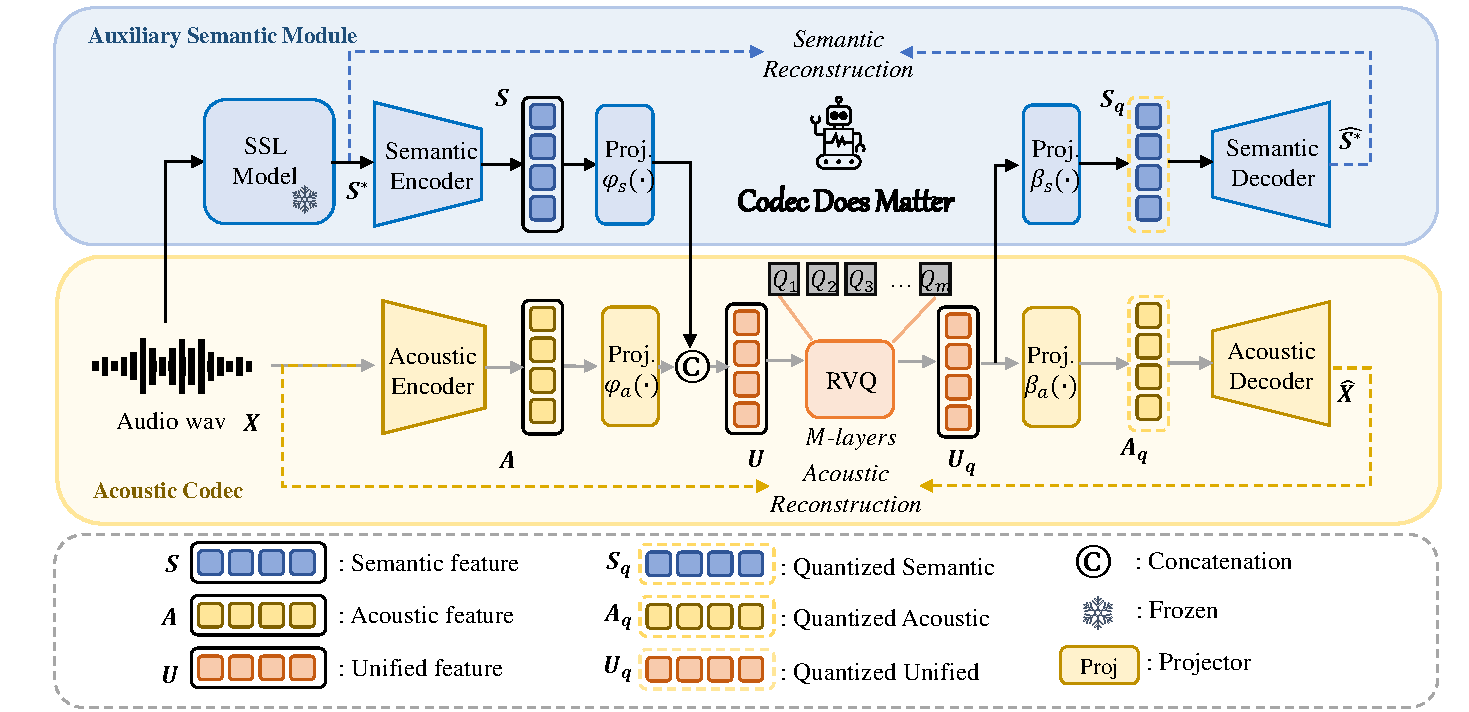
\includegraphics[scale=0.60]{imgs/fig1.pdf}
  \caption{The pipeline of X-codec.}
  \label{fig_xcodec}
\end{figure*}

\subsection{Audio Codec}

Recent advancements have seen a surge in deep learning methodologies employing vector quantization \cite{van2017neural} to reconstruct continuous signals into discrete representations for AR generation. Notably, audio codecs based on the VQ-GAN framework \cite{esser2021taming} have gained prominence. For example, SoundStream \cite{zeghidour2021soundstream} introduces a versatile codec adaptable to various audio types, integrating Residual Vector Quantization (RVQ) and Generative Adversarial Network (GAN) to refine quantization and reconstruction. Similarly, Encodec \cite{defossez2022high} enhances compression through a multi-scale discriminator and a loss-balancing strategy alongside a language model. HiFi-Codec \cite{yang2023hifi} employs Group-Residual Vector Quantization (GRVQ) to minimize the need for extensive codebooks while maintaining high reconstruction fidelity. DAC \cite{kumar2024high} addresses codebook collapse, where some codes remain unused, by applying improved codebook learning to achieve higher compression rates.


These codecs primarily focus on acoustic reconstruction and higher compression rates, often overlooking their potential as tokenizers for audio LLMs. Some attempts have been made to develop more suitable tokenizers for audio LLMs. For example, SpeechTokenizer \cite{zhang2023speechtokenizer} utilizes HuBERT to separate speech into distinct VQ components for content and timbre/acoustic details. This separation improves the modeling of content in the AR stage of VALL-E, while the NAR stage enriches the acoustic details. However, a distillation framework is exploited, this makes SpeechTokenizer may not be compatible with all LLM architectures, especially those that require uniform treatment of tokens, such as methods using flattened codec tokens \cite{yang2023uniaudio,copet2024simple}. Another attempt is presented by SemantiCodec \cite{liu2024semanticodec}, which employs a pre-trained AudioMAE \cite{huang2022masked} to generate distinct semantic and acoustic tokens from mel-spectrograms. However, this method inherits the issues of SpeechTokenizer and introduces additional complexity in token modeling. Moreover, since the audioMAE is performed on 2D time-frequency mel-spectrograms, LLMs must effectively handle dual scales (time and frequency), which may require significant modifications to existing LLM structures.

In contrast, our proposed X-Codec provides a uniform and comprehensive enhancement of semantic information for all tokens, resulting in significant performance improvements for existing audio LLMs without requiring any structural modifications. 

